\section{Lexical Functional Grammar}
{\tiny developed in the 80s by Joan Bresnan and Ron Kaplan, they view LFG as a psycholinguistically plausible alternative to transformation-based approaches, forms part of West-Coast linguistics}\\
\scriptsize{Untyped Feature Descriptions} {\tiny matrices that contain inflectional\\
problem: syncretism, the same form fills different cells in inflectional paradigms -> use disjuction (or statement)\\
embedding: one feature description might be embedded in another feature description\\
path: a sequence of features which immediately follow each other, e.g. derivational morphology\\
list: we can use a list of feature values (and statment)\\
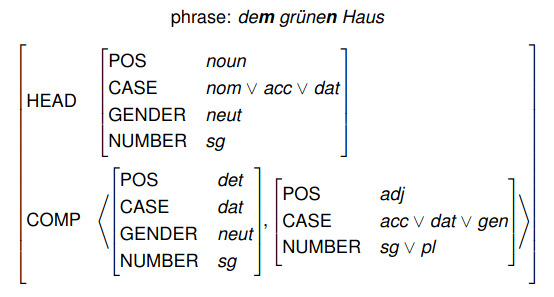
\includegraphics[scale=0.25]{untyped_feature_description.png}\\
}\\
\scriptsize{Typed Feature Descriptions} {\tiny i.e. feature structure, the type determines the template of feature labels that can be filled with values \\
inheritance: subordinate types inherit the features of their superordinate types\\
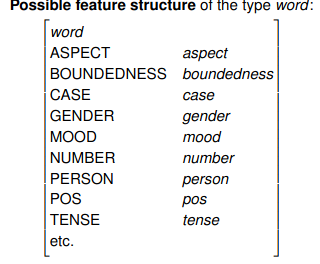
\includegraphics[scale=0.25]{type_word.png}\\
type hierarchies:\\
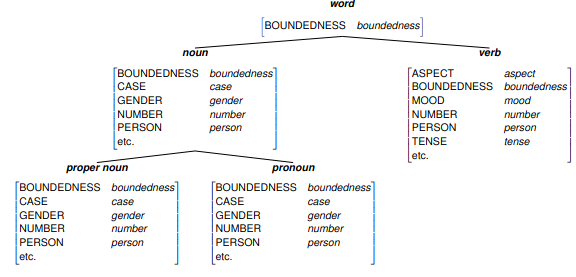
\includegraphics[scale=0.25]{type_hierarchy.png}
}\\
\scriptsize{Structure Sharing} {\tiny an identical feature structure is used in different parts of the feature description\\
e.g. agreement between determiner, adjective and noun in German:\\
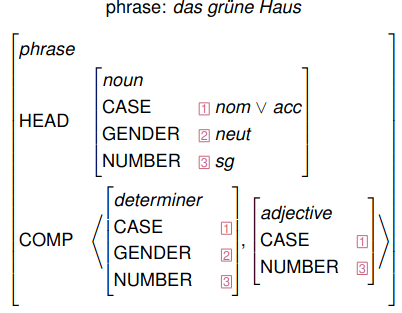
\includegraphics[scale=0.25]{agreement.png}\\
}
\scriptsize{Feature Descriptions and Structures}\\ 
{\tiny
A feature structure is a more general, stable model of all objects of a given type, while feature descriptions can give only (the relevant) parts of this model
}\\
\scriptsize{Grammatical Functions}\\ 
{\tiny e.g. PRED 'devour<SUBJ,OBJ>'}\\
\scriptsize{predicates (PRED)} 
{\tiny used for all lexical items that contribute meaning to the sentence, the value is either a lexical item(e.g.'David') or a lexical item followed by a list specifying grammatical functions (e.g.'devour<SUBJ,OBJ>')
}\\
{\scriptsize Syntactic Structure:\\
Argument Structure(A-Structure)
}\\
{\tiny general representation format: verb<x,y,z,ect.>\\
ordering: reflects a thematic hierarchy: agent>beneficiary>experiencer/goal>instrument>patient/theme>locative
}\\
\scriptsize{governable grammatical functions} 
{\tiny functions which have to be specidied by the head of the overall phrase/sentence\\
SUBJ, OBJ:object\\ $OBJ_{THEME}$:secondary object, direct object of a ditransitive sentence (e.g. gave \textit{the book}...)\\ COMP:sentential complement(that-clause)\\ OBL:oblique grammatical functions (e.g. $OBJ_{LOC}$: in..., at... after "located" (obligatory))
}\\
\scriptsize{non-governable grammatical functions} 
{\tiny functions that are not specidied by the head (not being arguments of the head)\\
ADJ(adjuncts), TOPIC, FOCUS(TOPIC and FOCUS can be used to model, e.g. word order variable when particular NPs are topicalized
}\\
\scriptsize{Functional Structure(F-Structure} 
{\tiny essentially a feature description for a whole phrase, e.g.:}\\
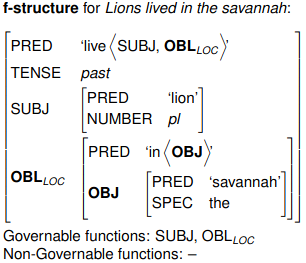
\includegraphics[scale=0.25]{f-structure1.png}\\
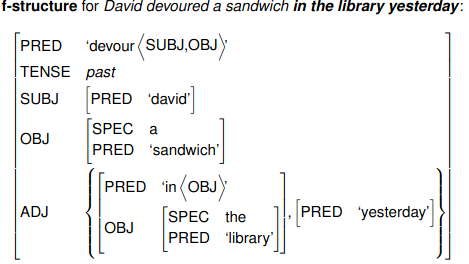
\includegraphics[scale=0.25]{f-structure3.png}\\
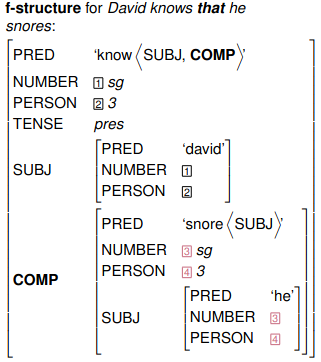
\includegraphics[scale=0.25]{f-structure2.png}\\
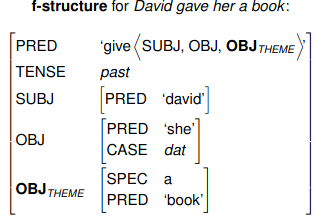
\includegraphics[scale=0.25]{f-structure4.png}\\
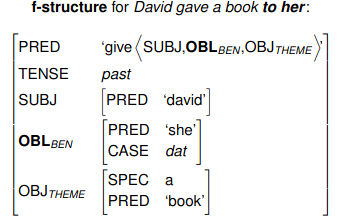
\includegraphics[scale=0.25]{f-structure5.png}\\
\scriptsize{Constituent Structure (C-Structure)} 
{\tiny licensed by (binary) phrase structure grammar, uses x-bar structures, e.g.:}\\
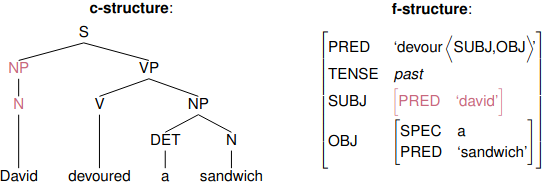
\includegraphics[scale=0.25]{c-structure1.png}\\
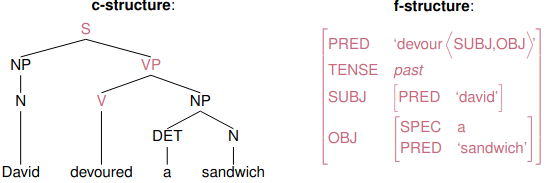
\includegraphics[scale=0.25]{c-structure2.png}\\
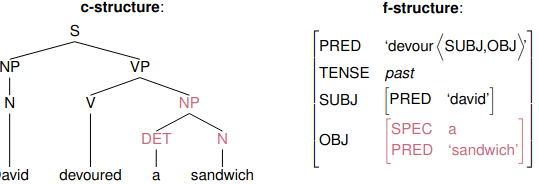
\includegraphics[scale=0.25]{c-structure3.png}\\
{\tiny summary: each structure models a different dimension of grammatical substance: role(a-structure), syntactic function(f-structure), phrase structure categories(c-structure)}\\
\scriptsize{Syntactic Phenomena\\
Passive} 
{\tiny simple mapping rule $verb<SBJ,OBJ> \to verb<(OBJ_{AG}),SBJ>$\\
translated into differing f-structures, valid for both configurational and non-configurational languages
}\\
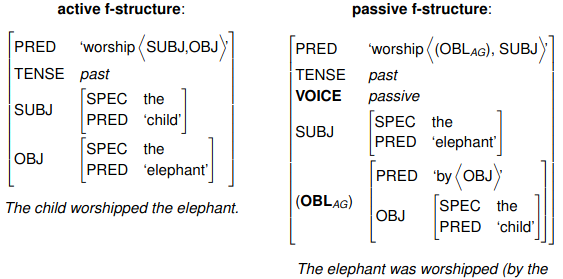
\includegraphics[scale=0.25]{LFG_passive.png}\\
\scriptsize{Pros} 
{\tiny fully formalized, computationally implementable\\
flexibility to deal with configurational(fixed word order) and non-configurational(flexible word order) languages\\
agreement and case assignment are modelled explicitely in the feature descriptions(similar to GPSG)\\
feature descriptions allow for analyses of long-distance dependencies and passive constructions without recurrence to transformations
}\\
\scriptsize{Cons} 
{\tiny Feature descriptions are untyped, which means that generalizations in terms of type hiearchies such as inheritance of features are not available (in contrast to HPSG)\\
the interactions between a-structure, f-structure, and c-structure are not straightforward, and will require a considerable amount of implementational details 
}